
\documentclass[11pt,letterpaper]{article}
\usepackage{naaclhlt2010}
\usepackage{paralist}
\usepackage{times}
\usepackage{latexsym}
\setlength\titlebox{6.5cm}    % Expanding the titlebox

\mathchardef\mhyp="2D

\title{Identifying Anomalous Activity the Enron Email \\
				Corpus using Glocal Multivariate Graph Statistics}

\author{Disa Mhembere\\
  Department of Computer Science\\
  Johns Hopkins University\\
  {\tt dmhembe1@jhu.edu}
  \And
  Kunal Lillaney \\
  Department of Computer Science\\
  Johns Hopkins University\\
  {\tt lillaney@jhu.edu}}

\date{}

\begin{document}
\maketitle
\begin{abstract}
Graphs are quickly emerging as a leading abstraction for the representation of data
flow and interactions within networks. One high-interest area of study deals with 
the use of graph theory to detect attacks and anomalous activity in networks 
\cite{priebe2005scan,park2009anomaly,park2013anomaly}.
Additionally, the use of machine learning to detect threats within networks 
has become a topic of particular interest 
\cite{mahoney2003machine,shon2005machine,sommer2010outside,shon2007hybrid} within
cyber security and machine learning circles alike.

The use of glocal multivariate graph statistics \cite{mhembere2013computing} as 
a supplementary source of multi-dimensional features for anomalous network detection,
has not been explored \textit{to our knowledge}. Such statistics can expose 
otherwise-latent topological attributes within networks that have the potential 
to improve abnormality detection within a network.

We use such statistics to generate novel features for use within
classification tasks for the Enron corpus of emails \cite{enronrepo2009}.
We hope to show that the use of such statistics can help to identify periods of
anomalous activity and those associated actors.
\end{abstract}


\section{Introduction}
% Problem
Detecting anomalies in order to expose malicious activity in networks is an
established problem within network security \cite{roesch1999snort,zhang2000intrusion}.
This problem is further exacerbated when one lacks data that constitutes what non-malicious
activity is represented as, within a specific network topology. This is the problem
we face when attempting to analyze the Enron email corpus. 

% Importance
Autonomous determination of network abnormality in addition to it source(s) is paramount
to many industries, including most notably, the finance industry.
Failure to monitor and detect such anomalies can lead to catastrophic financial
consequences for individuals and companies alike as demonstrated by the financial 
crisis of 2008 \cite{grigor2009financial}. A preventative measure is to develop automated tools
to determine when anomalous activity occurs within organizations and take action before
catastrophes occur. This work is a step toward developing such technologies.

% Difficulty
The unsupervised task of determining anomalous activity in data can be vastly more
complex than its supervised counterpart. Unfortunately, the choice of whether to use
a supervised or unsupervised method is primarily dictated by the data. The Enron email
corpus falls into the latter category and thus unsupervised learning is necessary.
The consequence is that we must now determine who may (or may not) be a malicious
actor without the concept/evidence of how `malicious' or `anomalous' is represented within
the data.

% Prior solutions ~ How we differ
Previously, many others have approached the problem by taking
samples of expected network activity and using these as a baseline for what is
normal \cite{chan2003machine,stein2005decision}. This is not feasible for our
particular dataset. We aim to instead produce supplementary features that potentially
highlight differences within the data.

% Key approach components and results (Limitaions)
We propose using a hybrid approach of graph theory and unsupervised machine learning.
Graphs are an intuitive high-level abstraction of interaction in any setting where
there is `information flow' and multiple points where its exchange may occur. As 
such, they naturally model email exchange. From derived graphs we obtain per-node
statistics which encode both local and global graph topological information. This
supplementary data can then be used to assist in classifying natively non-linear data.
This may have an analogous effect to the kernel trick used in non-linear 
classification in SVMs. %limitations
We should note that the computational cost of deriving a graph, given the
raw communication data, in addition to computing glocal graph statistics, may
be non-trial. As such, one might have to tradeoff such costs vs the number of graph
statistics computed.

\section{Background and Related Works}
In the early 2000's Chan et al \cite{chan2003machine} suggested non-bayesian 
learning algorithms that successfully avoided the zero-frequency problem i.e., determining
anomalous network activity given no prior samples. They propose the Learning rules for Anomaly
Detection (LERAD), a random sampling-based algorithm that attempts to learn anomaly
rules by bipartition feature-vectors and computing the probability of one feature set
partition to the other. The major drawback of this algorithm is the assumption that the 
training data is free from attacks which tends to be timely and difficult to rigorously
determine.

Chan et al \cite{chan2003machine} also developed Clustering for Anomaly Detection (CLAD).
On paper, this algorithm suits the type of classification we aim to do well. It is
essentially a variant of K-Nearest Neighbors, but has a more flexible parameter than K
for deciding the neighborhood that ultimately determines a samples label. By using a 
cluster width parameter, CLAD behaves like a flexible, per sample, K parameter, KNN.

Shon et al \cite{shon2007hybrid} proposed an unsupervised variant of the SVM, termed
the \textit{Enhanced SVM}. It reduces the false-positive rate and furthermore no longer required 
training data, as its characteristics resemble that of a one-class SVM. This method appears
reasonable, but is most effective with preprocessed data. The authors actually use 4 stages of
preprocessing and training before they run the actual SVM. This is an option that is 
not always available to some, like ourselves.

Others \cite{eskin2000anomaly} have attempted to model anomalies (and normal activity)
in sample data as a gaussian mixture(GMM) model. Here detection is simply a classifier that
discriminates on whether a sample could be generated by the GMM distribution or not.
This model unfortunately also assumes an initial portion of the data is anomaly free.
Though the Enron corpus may generally be modeled with this assumption, we cannot
determine whether this is truly accurate. There is a further persistent assumption
that anomalies are `rare' by necessity with such algorithms. Such an algorithm is also
prone to mis-classification as it performs best on linearly-separable data.

Stein et al \cite{stein2005decision} proposed minimizing the feature-space used for 
anomaly detection by using genetic algorithms to solve the optimization problem of which
features best classify the anomalous activity. This method has the disadvantage of requiring
labelled data in order to train a supervised learning algorithm.

Finally, others have applied self-organizing maps \cite{rhodes2000multiple}, fuzzy logic \cite{zimmermann1992fuzzy}, neural networks \cite{mukkamala2002intrusion} and more to 
solve intrusion detection problems which are a near-equivalent class of problems to anomaly detection.

\section{Design}
This section describes our choice of glocal graph statistics and discusses their suitability
to the task of detection of anomalous activity and anomalous actors in the Enron email corpus.
We further discuss our choice of Machine Learning algorithms. Lastly, we discuss our metrics
of success and evaluation for our implementations.

\subsection{Graph Statistics} \label{graph_stats}
Carey et al \cite{priebe2005scan} showed that through the use of the a glocal graph 
statistic (namely the Scan statistic), one could successfully detect anomalous activity.
We choose to look further and ask whether traditional topologically-encoded graph statistics would
be even better suited to the task of classifying both periods of anomaly and those
most highly associated with the anomaly.

For consistency, let $G$ be a graph, with vertex set $V$ and edges $u \sim v \in E$ (the set of
all $m$ edges). Let $e_{ij}$ be a directed edge from $v_i$ to $v_j$. Let $l(u,v)$ be the edge
distance between vertices $u, v$. Let the $k$-hop \emph{neighborhood} of a graph $G$ around
vertex $v$ be denoted by $N_k[v;G]$, where $N_k[v;G] = \{u \in V:l(u,v) \le k\}$. Let $\eta_i$ 
denote the neighbors for $v_i$. Finally, let the $C\mhyp k$ denote the size of a clique as $k$, where a clique $C \subset V$ s.t $\forall\ v,u \in C\ \exists\ v \sim u$.

 
As such we use the following statistics:
\begin{itemize}
\item Local in-degree: $deg_{in} = \sum_{j \in \eta_i} v_{ji}\  \forall\ v \in V$
\item Local out-degree: $deg_{out} = \sum_{j \in \eta_i} v_{ij}\  \forall\ v \in V$ 
\item Local triangle count: $\Delta = C\mhyp3 \  \forall\ v \in V$
\item Local scan-1 statistic: \\ $SS = \sum e_{ij} \in N_1[v_i;G] \forall\ v \in V$
\item Local clustering coefficient: \\ Let, $deg = deg_{in} + deg_{out}$ 
\\ $CC = \frac{2\Delta}{deg (deg-1)}$
\item Eigen-spectral decomposition: $\lambda = \mathbf{vA}$, where $\lambda$ are the
eigenvalues, $\mathbf{v}$ are the eigenvectors, and $\mathbf{A}$ is the adjacency matrix of $G$.

\end{itemize}
These statistics have proved extremely statistically powerful in summarizing graph
topology \cite{pao2011statistical}. All but Eigen-spectral decomposition provide
connectivity and interaction information from one vertex to the next. These will
logically be the most informative in our case since we hypothesize there is a strong
correlation between topological non-homogeneity within graphs and anomalous/malicious
activity. The spectral decomposition actually produces a condensed relationship mapping
between each pair of vertices in the graph. As such, it follows that this is an obvious
candidate for determining when atypical patterns occur in the graph.

\subsection{Machine Learning Tools}
\hspace*{10pt}\textit{Anomalous time periods:} \\
One aim is to determine \textit{when} atypical communications occur. We choose to
use weighted k-Nearest Neighbors (wKNN) to identify malicious actors in the network
at different time points since we conjecture the features of malicious users will
have high relative \textit{similarity}, where we use feature-vector squared euclidean distance
as our metric for similarity. i.e.,

$d = \sqrt{\sum\limits_{i=1}^N s_i (x_i = x_i')^2 }$


\textit{Anomalous actors:} \\
The other aim is to deterrine \textit{who} were those who caused the anomalous
activity during these periods of unrest. Literature \cite{shon2007hybrid,shon2005machine}
leads us to believe that Support Vector Machines (SVM)s are a suitable from such 
a classification task. *Unfortunately, time did not permit us to implement this.


\section{Methods}
In this section we describe both the data acquisition phase and the learning algorithm
implementation and the challenges we faced in the pursuit of both.

\subsection{Data Acquisition}
To realize our goals we obtain raw data from two sources:
\begin{inparaenum}[\itshape(i)]
\item http://www.cs.cmu.edu/$\sim$./enron/. This resource contains over 0.5 million
emails from senior management within Enron and 
\item http://cis.jhu.edu/parky/Enron/enron.html. This is a resource from where we obtain
time-series graphs of Enron email activity for a 189 week period between 1998 and 2002.
Here each graph represents a week of email interaction between $\sim$150 to executives
at Enron.
\end{inparaenum}

\subsubsection{Raw email Feature Extraction}
We used the raw email data to derive $18$ frequency based features. The feature set
included the following: 
\begin{itemize} \itemsep0em
\item Sent/Received emails (In network and out)
\item Sent/Received CC emails (In network and out)
\item Sent/Received BCC emails (In network and out)
\item Sent/Received mean email length
\item Sent/Received on weekday (Mon-Fri)  (In network and out)
\item Sent/Received on weekend (Sat,Sun)  (In network and out)
\item Sent/Received during business hours (8a.m - 6p.m) (In network and out)
\item Sent/Received outside business hours (8a.m - 6p.m) (In network and out)
\end{itemize}

We define `in network' as emails sent from and to the same domain e.g 
\texttt{sender@domainX.com} to \texttt{recepient@domainX.com}, and out of network'
as emails sent from one domain to another that is not the same e.g \texttt{sender@domainX.com}
to \texttt{recepient@domainY.com}.


\subsubsection{Challenges: Raw email Feature Extraction}
We faced several challenges while accumulating feature vectors:
\begin{itemize} \itemsep0em
\item Several email addresses link to a single user. We did not solve this issue as it is
impossible determine a mapping of email addresses to names since a name is non-unque.
\item Non-uniform email addresses generated in raw text. Due to \textit{smart} email clients
some email addresses were given aliases in the form of nicknames. We did not attempt to
solve this.
\item Auto-generated emails. Some emails were generated by the email clients to certain
users. This is the case for \textit{Reminder} emails. We choose to ignore these.
\end{itemize}


\subsubsection{Time Series Feature Extraction}
We used the igraph \cite{igraph2006} package to generate the 6 glocal graph statistics
described in section \ref{graph_stats}. Note that the time series graphs only contained 
$\sim$ 190 of the most influential Enron employees, whereas the feature vectors we produced
for classification include all senders and recipients inside and outside Enron who totaled $86,857$.
We write the feature vector instances in batches of weeks to match the time series graphs.
This means the same user is potentially represented up to once for each week of emails sent.

\subsubsection{Regularization}
In order ensure no single features raw magnitude dictated the classification task we performed
regularization by ensuring the standard deviation of the every feature vector was equal to 1.
We achieved this via the sci-kit learn \cite{scikit-learn} library.

\section{Experiment Design}

\hspace*{10pt}\textit{Anomalous actors:} \\
We first run the distance Weighted KNN on instances with no graphs statistics, then we
repeat the experiment on instances that do contain graph statistics. We do this to gauge
the improvement in classification.

We previously accumulated a list of Enron employees convicted and now manually determine
whether these individuals are clustered together.
	
\hspace*{10pt}\textit{Anomalous time periods:} \\
**NOT DONE: Since we store the feature-vector instances by the week we are able to note when one individual
moves from a \textit{normal} cluster to an \textit{anomalous} one. Weeks with the highest
number of these switches are noted as anomalous time periods.

\section{Results}

\begin{tabular}{cc}
  \num\putindeepbox[7pt]{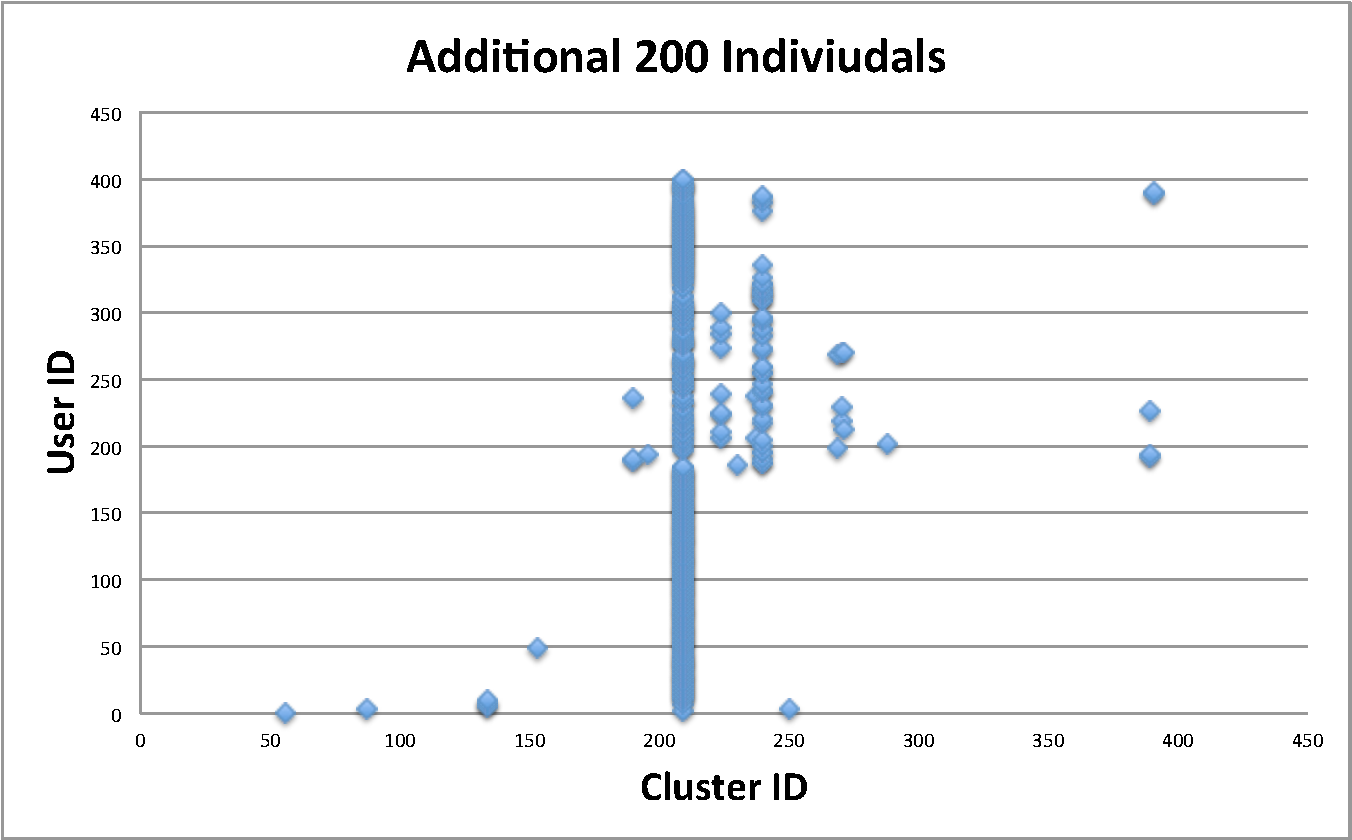
\includegraphics{img200inv.pdf}}
  & \num\putindeepbox[7pt]{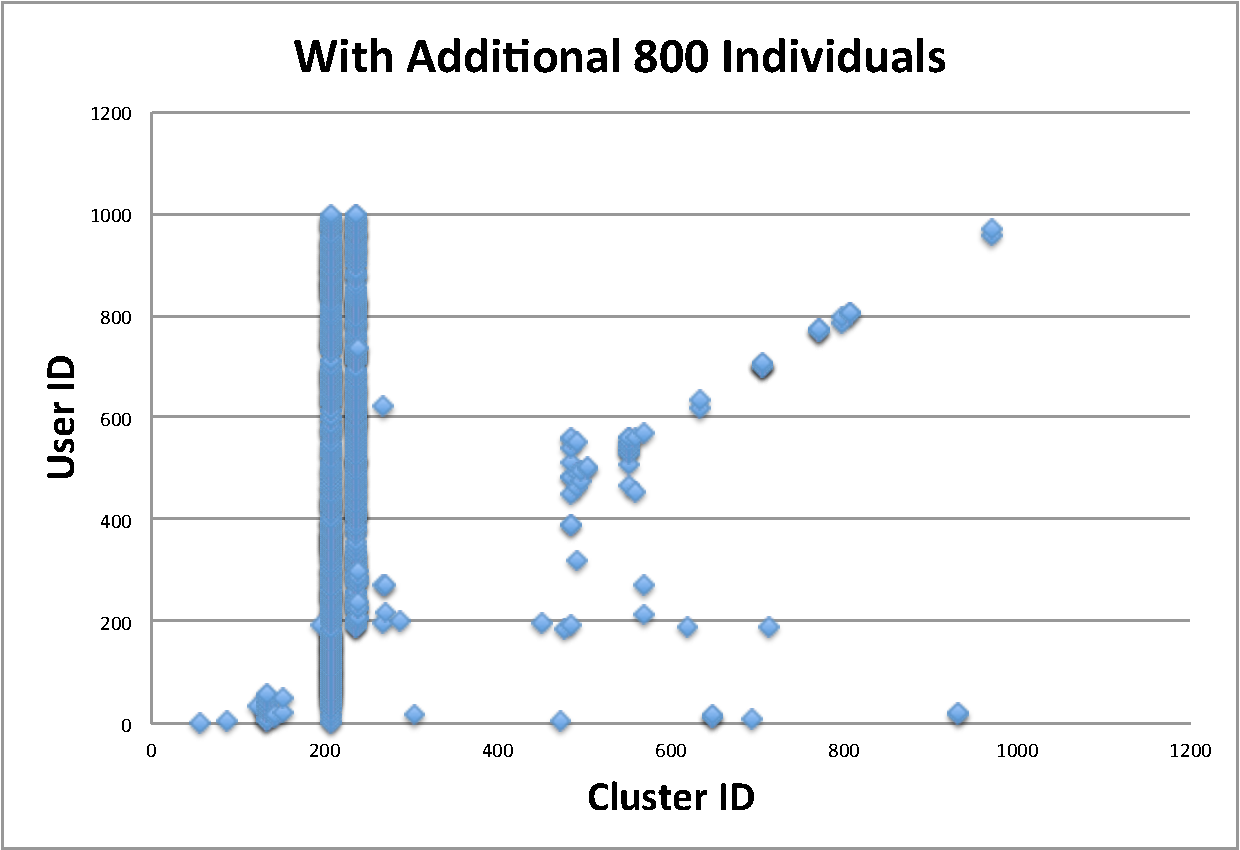
\includegraphics{img800inv.pdf}} \\
  \num\putindeepbox[7pt]{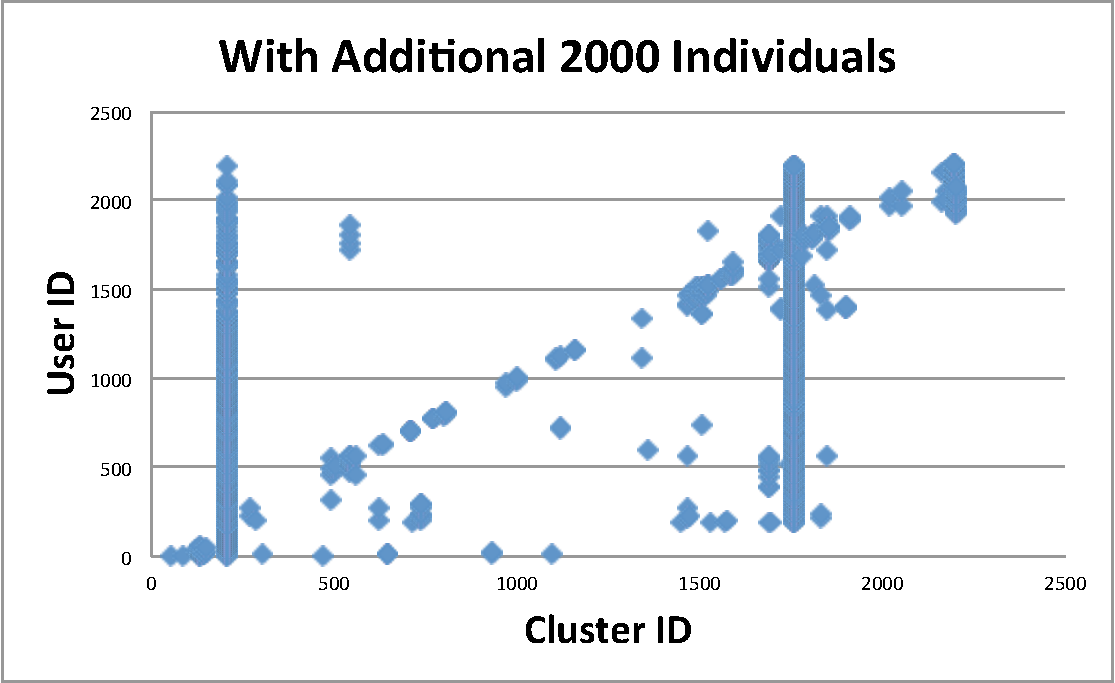
\includegraphics{img2000inv.pdf}}
  & \num\putindeepbox[7pt]{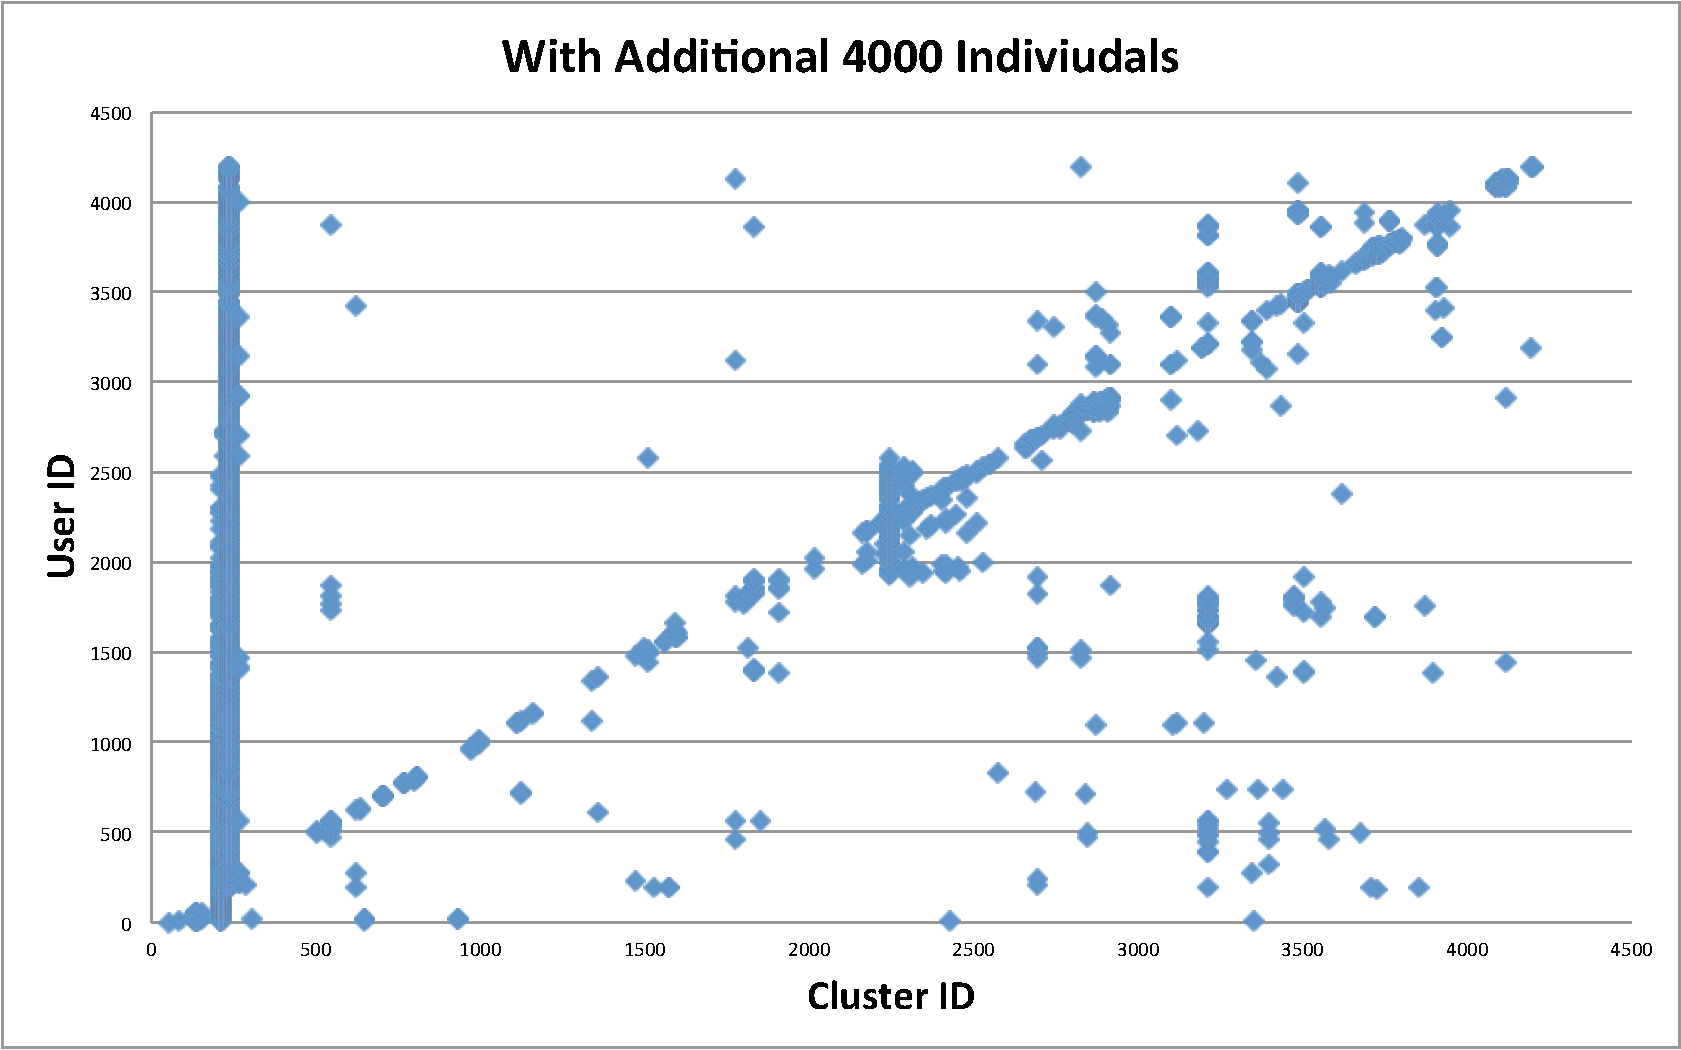
\includegraphics{img4000inv.pdf}} \\
\end{tabular}

- Run with no invariants \\

- Run with invariants \\

- Number of switches per week \\


No computational time to classify time periods

Analysis of the results: \\

Reasons for ineffectiveness: \\

- Features may not match what we want to cluster for \\
- Sparse \\ 
- Very expensive to train wKNN and more complex classifiers e.g SVM \\

\section{Comparison to proposal}
We achieved most of what we set out accomplish! Time did not permit the implementation of
a one-class SVM to classify time periods of anomaly, but can infer this information from
the weighted KNN results.

\section*{Bibliography}
\bibliographystyle{ieeetr}
\bibliography{writeup.bib}
%\bibliographystyle{acl}
%\bibliography{references.bib}
\end{document}
